% ============================================================
% Unidade 04 — Variáveis Ambientais e Multicolinearidade
% ============================================================

\chapter{Variáveis Ambientais e Multicolinearidade}

\section*{Abertura da Unidade}

A modelagem de distribuição de espécies depende de três pilares fundamentais: registros biológicos confiáveis, uma área acessível biologicamente coerente e variáveis ambientais capazes de representar, de forma ecologicamente interpretável, as condições que limitam ou favorecem a presença das espécies. Nas unidades anteriores, discutimos a distribuição das espécies como resultado da interação entre nicho ecológico, história biogeográfica, acessibilidade e qualidade dos registros biológicos. Nesta unidade, avançamos para o terceiro componente essencial da modelagem: a escolha criteriosa das variáveis ambientais. Essa etapa é central porque os modelos de distribuição não acessam diretamente o nicho ecológico; eles estimam relações entre ocorrências observadas e gradientes ambientais mensurados no espaço geográfico \parencite{hutchinson1957concluding,elith2009species}.

Em Modelagem de Distribuição de Espécies, as variáveis ambientais funcionam como descritores mensuráveis do componente abiótico do nicho. Elas traduzem, para o espaço geográfico, gradientes de temperatura, precipitação, sazonalidade, relevo, solos e outros fatores que podem influenciar a ocorrência, o crescimento, a sobrevivência e a reprodução das espécies. No framework BAM, essas variáveis representam principalmente o componente \textit{A}, isto é, o conjunto de condições abióticas sob as quais uma espécie pode manter populações viáveis \parencite{soberon2007grinnellian,peterson2011ecological}. Assim, a escolha inadequada dessas variáveis pode comprometer todo o processo de modelagem, mesmo quando os dados de ocorrência foram cuidadosamente limpos e a área \textit{M} foi bem delimitada.

Para espécies arbóreas amazônicas como \textit{Dinizia excelsa} Ducke, essa etapa é particularmente importante. A espécie ocorre em uma região ambientalmente heterogênea, marcada por variações climáticas, edáficas, geomorfológicas e biogeográficas. Portanto, representar seu nicho apenas com um conjunto automático de variáveis climáticas pode produzir modelos estatisticamente satisfatórios, mas ecologicamente frágeis. A seleção de variáveis deve combinar conhecimento ecológico, interpretação ambiental, critérios estatísticos e atenção à multicolinearidade, evitando que o modelo seja conduzido apenas por padrões numéricos sem significado biológico claro \parencite{franklin2010mapping,guisan2017habitat}.

Após a delimitação da área acessível, discutida na Unidade 03, o próximo passo consiste em caracterizar ambientalmente essa região. Em outras palavras, uma vez definido o espaço geográfico que a espécie poderia ter alcançado ao longo de sua história biogeográfica, torna-se necessário compreender quais gradientes ambientais estruturam seu nicho ecológico dentro desse espaço. Assim, a seleção de variáveis ambientais representa a ponte entre o componente \textit{M} do framework BAM, a construção de pseudo-ausências e background na Unidade 05 e os algoritmos de modelagem que serão apresentados nas Unidades 06 a 11.

\begin{figure}[H]
	\centering
	\includegraphics[width=0.92\textwidth]{figuras/unidade04/unidade04_nicho_variaveis_ambientais.png}
	\caption{Relação conceitual entre nicho ecológico, gradientes ambientais, variáveis ambientais e modelos de distribuição de espécies. As variáveis ambientais não representam o nicho em si, mas aproximações mensuráveis de condições ecológicas relevantes para a espécie.}
	\label{fig:unidade04_nicho_variaveis}
\end{figure}

\section*{Objetivos da Unidade}

Ao final desta unidade, espera-se que o leitor seja capaz de compreender o papel das variáveis ambientais na representação do nicho ecológico; reconhecer as principais fontes de dados ambientais utilizadas em SDM; distinguir variáveis climáticas, topográficas e edáficas; compreender o problema da correlação e da multicolinearidade; aplicar critérios estatísticos e ecológicos para selecionar variáveis; interpretar matriz de correlação, VIF e PCA; e construir um conjunto ambiental ecologicamente coerente para modelar a distribuição de \textit{Dinizia excelsa} na Amazônia.

\section{O Papel das Variáveis Ambientais em SDM}

A distribuição das espécies não ocorre ao acaso no espaço geográfico. Ela reflete, em diferentes escalas, a interação entre condições ambientais, história evolutiva, dispersão, interações bióticas e processos demográficos. Em SDM, as variáveis ambientais são utilizadas para representar parte dessa complexidade, especialmente os gradientes abióticos que definem onde uma espécie pode manter populações viáveis. Essa lógica deriva diretamente da tradição grinnelliana do nicho, na qual o nicho é compreendido a partir das condições ambientais que regulam a presença da espécie no espaço \parencite{grinnell1917niche,soberon2007grinnellian}.

A tradição hutchinsoniana ampliou essa interpretação ao formalizar o nicho como um hipervolume multidimensional, no qual cada dimensão representa uma condição ou recurso relevante para a persistência da espécie. Sob essa perspectiva, variáveis ambientais como temperatura, precipitação, sazonalidade e atributos do solo são dimensões observáveis, ainda que simplificadas, desse hipervolume ecológico. Portanto, ao construir um modelo de distribuição, o pesquisador está projetando parte desse espaço ambiental no espaço geográfico \parencite{hutchinson1957concluding,peterson2011ecological}.

No framework BAM, as variáveis ambientais descrevem principalmente o componente \textit{A}, isto é, o conjunto de condições abióticas adequadas à espécie. Entretanto, é fundamental reconhecer que o modelo não observa diretamente o nicho ecológico. Ele observa associações entre registros de ocorrência e valores ambientais disponíveis em células espaciais. Assim, as variáveis ambientais são aproximações mensuráveis de processos ecológicos mais complexos, e sua interpretação deve ser sempre feita à luz da biologia da espécie e da escala espacial do estudo \parencite{soberon2007grinnellian,guisan2017habitat}.

Para \textit{Dinizia excelsa}, variáveis como temperatura, precipitação, sazonalidade climática, altitude, relevo e atributos edáficos podem estar relacionadas a processos fundamentais, como tolerância hídrica, disponibilidade de água no solo, produtividade florestal, estresse climático, estabilidade ambiental e restrições fisiológicas. O objetivo da seleção ambiental não é simplesmente maximizar métricas como AUC ou TSS, mas construir um espaço ambiental coerente com a ecologia da espécie. Esse princípio é especialmente importante quando o modelo será usado para projeções futuras, pois variáveis mal escolhidas podem comprometer a transferibilidade espacial e temporal \parencite{elith2009species,zurell2020standard}.

\begin{caixaconceitual}{Variável ambiental não é apenas uma coluna da tabela}
	Em SDM, uma variável ambiental deve ser entendida como uma hipótese ecológica espacializada. Ao incluir precipitação anual, assume-se que a disponibilidade hídrica média pode influenciar a distribuição da espécie. Ao incluir sazonalidade da precipitação, assume-se que a variação intra-anual da água pode ser relevante. Portanto, selecionar variáveis é também selecionar hipóteses ecológicas sobre o nicho.
\end{caixaconceitual}

Um erro comum em SDM é tratar variáveis ambientais como simples preditores estatísticos. Essa prática pode gerar modelos com bom desempenho aparente, mas com baixa interpretabilidade e reduzida capacidade de transferência para outros períodos, regiões ou cenários climáticos. Modelos construídos com variáveis redundantes, pouco interpretáveis ou ecologicamente desconectadas da espécie tendem a ser frágeis quando projetados para o futuro ou para áreas externas à calibração \parencite{araujo2005validation,thuiller2004effects}.

\section{Principais Fontes de Variáveis Ambientais}

A expansão da modelagem de distribuição de espécies foi fortemente impulsionada pela disponibilidade de bases ambientais globais. Entre as mais utilizadas estão WorldClim, CHELSA, TerraClimate, SoilGrids, EarthEnv e ENVIREM. Cada uma dessas bases possui objetivos, resoluções, métodos de interpolação e limitações específicas. A escolha da fonte deve considerar a escala do estudo, a ecologia da espécie, a resolução dos dados de ocorrência e o objetivo da modelagem \parencite{franklin2010mapping,guisan2017habitat}.

\subsection{WorldClim}

O WorldClim é uma das bases climáticas mais utilizadas em SDM. Ele disponibiliza camadas de temperatura e precipitação, incluindo variáveis bioclimáticas derivadas de médias, extremos e sazonalidade. Sua ampla utilização decorre da cobertura global, da facilidade de acesso e da compatibilidade com pacotes em R usados em modelagem ecológica. No entanto, em regiões tropicais remotas, como partes da Amazônia, a densidade desigual de estações meteorológicas pode afetar a precisão das interpolações climáticas \parencite{fick2017worldclim,booth2014bioclim}.

As variáveis bioclimáticas do WorldClim são especialmente úteis porque sintetizam aspectos ecológicos do clima, como temperatura média anual, sazonalidade térmica, precipitação do trimestre mais seco e precipitação do trimestre mais chuvoso. Essas variáveis frequentemente apresentam maior significado biológico do que médias mensais isoladas, pois capturam condições médias, limites e extremos potencialmente relevantes para a distribuição das espécies \parencite{booth2014bioclim,guisan2017habitat}.

\subsection{CHELSA}

A base CHELSA também fornece dados climáticos globais, mas utiliza procedimentos de downscaling que buscam representar melhor efeitos orográficos e padrões atmosféricos. Em áreas montanhosas ou com forte influência topográfica, essa abordagem pode oferecer vantagens em relação a bases climáticas mais generalistas. Para a Amazônia de baixa altitude, sua utilidade deve ser avaliada em função da escala do estudo, da resolução desejada e da coerência entre os dados climáticos e os registros de ocorrência \parencite{karger2017climatologies}.

O uso de CHELSA pode ser particularmente relevante em estudos que envolvem gradientes altitudinais, transições entre planaltos e áreas de baixada ou regiões de relevo complexo. Entretanto, assim como em qualquer base ambiental, sua inclusão deve ser orientada por perguntas ecológicas claras. A substituição automática de uma base por outra não garante melhoria do modelo se a escala, a incerteza e o significado biológico das variáveis não forem considerados \parencite{elith2009species,zurell2020standard}.

\subsection{TerraClimate}

O TerraClimate combina informações climáticas de diferentes fontes para produzir séries temporais mensais de variáveis como temperatura, precipitação, evapotranspiração e balanço hídrico. Essa base é especialmente útil quando o interesse envolve variação temporal, tendências climáticas ou reconstruções anuais e mensais. Em estudos de SDM, pode ser relevante para modelagens dinâmicas ou análises associadas a secas, déficit hídrico e mudanças climáticas recentes \parencite{abatzoglou2018terraclimate}.

Para espécies arbóreas tropicais, variáveis relacionadas ao balanço hídrico podem representar processos ecológicos mais diretamente do que a precipitação isolada. A evapotranspiração, a disponibilidade de água no solo e indicadores de déficit hídrico podem estar associados ao crescimento, mortalidade e vulnerabilidade a eventos extremos. Assim, o TerraClimate pode complementar bases bioclimáticas clássicas quando o objetivo envolve dinâmica climática, seca ou risco climático \parencite{franklin2010mapping,guisan2017habitat}.

\subsection{SoilGrids}

O SoilGrids fornece informações edáficas globais, incluindo textura, carbono orgânico, pH, densidade do solo e outras propriedades. Para espécies arbóreas tropicais, variáveis de solo podem ser fundamentais, pois influenciam disponibilidade de nutrientes, retenção de água, drenagem, crescimento radicular e produtividade. Contudo, a resolução e a incerteza desses produtos devem ser avaliadas com cuidado, sobretudo em regiões com baixa densidade de amostras de solo \parencite{poggio2021soilgrids}.

A inclusão de variáveis edáficas em SDM deve ser feita de forma crítica. Em muitos casos, os produtos globais de solo apresentam incerteza espacial considerável, mas isso não significa que o solo deva ser ignorado. Para plantas, especialmente árvores de grande porte, os atributos edáficos podem ser determinantes importantes da distribuição local e regional. O desafio consiste em equilibrar relevância ecológica, qualidade espacial dos dados e interpretabilidade do modelo \parencite{guisan2017habitat,franklin2010mapping}.

\subsection{EarthEnv}

A iniciativa EarthEnv disponibiliza diferentes camadas ambientais globais, incluindo produtos derivados de relevo, cobertura da terra, habitat e sensoriamento remoto. Essas variáveis podem ser úteis para complementar informações climáticas e edáficas, especialmente quando se deseja representar heterogeneidade ambiental, estrutura de habitat ou gradientes topográficos. Em SDM, sua utilidade depende da relação entre a variável, a ecologia da espécie e a escala espacial da modelagem \parencite{tuanmu2014global}.

No caso de espécies florestais amazônicas, variáveis derivadas de relevo e habitat podem funcionar como substitutos de processos locais, como drenagem, posição topográfica, heterogeneidade de paisagem e condições microclimáticas. Entretanto, o pesquisador deve evitar incluir variáveis de difícil interpretação ecológica apenas porque estão disponíveis. A abundância de dados ambientais não elimina a necessidade de uma hipótese ecológica explícita \parencite{elith2009species,zurell2020standard}.

\subsection{ENVIREM}

O ENVIREM disponibiliza variáveis ambientais derivadas com forte interpretação ecológica, incluindo descritores relacionados à aridez, sazonalidade, energia ambiental e disponibilidade hídrica. Essas variáveis foram desenvolvidas para ampliar a representação ambiental em estudos de distribuição de espécies e podem ser úteis quando se deseja incluir dimensões do ambiente não capturadas adequadamente pelas variáveis bioclimáticas tradicionais \parencite{title2018envirem}.

Em projeções futuras ou estudos comparativos, variáveis derivadas como índices de aridez e sazonalidade podem auxiliar na interpretação de respostas ecológicas a mudanças climáticas. Contudo, sua inclusão deve ser acompanhada de avaliação de correlação, redundância e significado biológico. Assim como ocorre com as variáveis do WorldClim, muitas variáveis derivadas podem estar fortemente correlacionadas entre si, exigindo procedimentos de seleção cuidadosos antes da modelagem \parencite{guisan2017habitat,zurell2020standard}.

\begin{table}[H]
	\centering
	\caption{Principais fontes de variáveis ambientais utilizadas em Modelagem de Distribuição de Espécies.}
	\label{tab:fontes_variaveis_ambientais}
	\small
	\begin{tabular}{p{2.6cm}p{3.0cm}p{3.5cm}p{3.5cm}p{3.5cm}}
		\toprule
		\textbf{Base de dados} & \textbf{Tipo de informação} & \textbf{Vantagens} & \textbf{Limitações} & \textbf{Uso recomendado em SDM} \\
		\midrule
		WorldClim & Temperatura, precipitação e variáveis bioclimáticas & Ampla cobertura, fácil acesso e uso consolidado em SDM & Incertezas em regiões com baixa densidade de estações meteorológicas & Modelos climáticos gerais e comparáveis \\
		CHELSA & Clima interpolado com downscaling & Melhor representação de efeitos orográficos e atmosféricos & Processamento mais complexo e necessidade de avaliação local & Estudos em áreas topograficamente heterogêneas \\
		TerraClimate & Séries temporais climáticas e balanço hídrico & Útil para dinâmica temporal, seca e variabilidade climática & Resolução e agregação temporal devem ser compatíveis com o objetivo & Análises de secas, tendências e variação temporal \\
		SoilGrids & Propriedades físicas e químicas do solo & Inclui atributos edáficos relevantes para plantas & Incerteza espacial pode ser alta em regiões pouco amostradas & Espécies sensíveis a solos, drenagem e fertilidade \\
		EarthEnv & Topografia, habitat e sensoriamento remoto & Grande diversidade de descritores ambientais & Algumas variáveis têm interpretação ecológica indireta & Complementar clima com estrutura ambiental e habitat \\
		ENVIREM & Variáveis ecologicamente derivadas & Forte interpretação ecofisiológica e climática & Requer seleção cuidadosa por correlação e redundância & Estudos com hipóteses sobre energia, aridez e sazonalidade \\
		\bottomrule
	\end{tabular}
\end{table}

\begin{caixaatencao}{Mais variáveis não significam melhor modelo}
	A inclusão indiscriminada de muitas variáveis ambientais aumenta o risco de redundância, multicolinearidade, sobreajuste e baixa transferibilidade. Em SDM, a parcimônia é uma virtude científica: modelos mais simples, quando ecologicamente bem fundamentados, frequentemente são mais robustos, interpretáveis e transferíveis.
\end{caixaatencao}

\section{Variáveis Climáticas}

As variáveis climáticas são os preditores mais utilizados em SDM porque o clima exerce forte controle sobre a distribuição das espécies em escalas regionais, continentais e globais. Temperatura e precipitação influenciam metabolismo, fenologia, balanço hídrico, produtividade primária, mortalidade, regeneração e limites fisiológicos. Para plantas, esses efeitos são particularmente relevantes, pois a ocorrência de uma espécie depende da capacidade de completar seu ciclo de vida sob determinadas condições de energia e água \parencite{woodward1987climate,franklin2010mapping}.

\subsection{Temperatura}

Variáveis de temperatura representam gradientes térmicos médios, extremos e sazonais. Em florestas tropicais úmidas, a temperatura média anual pode variar menos do que em regiões temperadas, mas pequenas diferenças térmicas podem estar associadas à altitude, continentalidade, estresse fisiológico e mudanças no balanço de vapor d’água da atmosfera. Além disso, temperaturas máximas e mínimas podem afetar eventos críticos, como estresse térmico, respiração, germinação e sobrevivência de plântulas \parencite{guisan2017habitat,booth2014bioclim}.

Em projeções de mudanças climáticas, variáveis térmicas assumem papel ainda mais importante. O aumento da temperatura pode deslocar envelopes climáticos, intensificar déficit de pressão de vapor e alterar a disponibilidade hídrica efetiva, mesmo quando a precipitação anual não muda substancialmente. Portanto, interpretar temperatura apenas como média anual pode ser insuficiente para compreender respostas ecológicas de espécies arbóreas tropicais \parencite{thuiller2004effects,zurell2020standard}.

\subsection{Precipitação}

Variáveis de precipitação representam disponibilidade hídrica, regime de chuvas e sazonalidade. Na Amazônia, a quantidade anual de chuva é importante, mas a distribuição ao longo do ano pode ser ainda mais relevante. Duas áreas com precipitação anual semelhante podem diferir fortemente na duração da estação seca. Para árvores de grande porte, esse aspecto pode afetar disponibilidade de água no solo, risco de embolia hidráulica, crescimento radial e mortalidade durante eventos extremos \parencite{nepstad2007amazon,phillips2009drought}.

A precipitação também deve ser interpretada em conjunto com relevo, solo e evapotranspiração. Uma área com alta precipitação anual pode apresentar déficit hídrico sazonal se os solos forem rasos, arenosos ou pouco capazes de armazenar água. Por outro lado, solos profundos e bem estruturados podem amortecer períodos secos. Em SDM, essa interação mostra que variáveis climáticas raramente atuam de forma isolada; elas se combinam com outros componentes ambientais para definir condições de adequabilidade \parencite{franklin2010mapping,guisan2017habitat}.

\subsection{Sazonalidade climática}

A sazonalidade climática descreve a variação intra-anual da temperatura e da precipitação. Em SDM, variáveis sazonais podem capturar diferenças entre ambientes climaticamente estáveis e ambientes com maior oscilação anual. Para espécies amazônicas, a sazonalidade da precipitação pode funcionar como filtro ecológico importante, especialmente em regiões de transição entre florestas úmidas, florestas estacionais e formações mais abertas \parencite{booth2014bioclim,terborgh1973distribution}.

Em árvores tropicais, a sazonalidade pode influenciar fenologia, germinação, recrutamento, crescimento cambial e mortalidade. Portanto, variáveis como precipitação do trimestre mais seco, precipitação do trimestre mais quente e sazonalidade da precipitação podem apresentar significado ecológico maior do que a precipitação anual total. Essas variáveis ajudam a representar períodos críticos, nos quais a sobrevivência ou o crescimento podem ser limitados \parencite{guisan2017habitat,elith2009species}.

\subsection{Extremos climáticos}

Extremos climáticos merecem atenção especial. Médias anuais podem ocultar eventos críticos que controlam a presença ou ausência de uma espécie. Uma árvore pode tolerar determinada precipitação média, mas não sobreviver a longos períodos de déficit hídrico extremo. Por isso, variáveis relacionadas ao trimestre mais seco, ao mês mais quente ou à sazonalidade podem ser biologicamente mais informativas do que médias simples \parencite{phillips2009drought,zurell2020standard}.

Em cenários de mudanças climáticas, os extremos podem ser mais relevantes do que as médias para explicar perdas de adequabilidade. Eventos de seca severa, ondas de calor e alterações na duração da estação seca podem modificar a distribuição potencial de espécies florestais, especialmente aquelas associadas a ambientes úmidos e climaticamente estáveis. Assim, a escolha de variáveis climáticas deve considerar não apenas o clima médio atual, mas também os mecanismos pelos quais extremos climáticos podem limitar a persistência das populações \parencite{thuiller2004effects,araujo2005validation}.

\begin{caixaaplicacao}{Clima e \textit{Dinizia excelsa}}
	Para \textit{Dinizia excelsa}, variáveis climáticas devem ser interpretadas à luz da ecologia de uma árvore emergente amazônica. A espécie pode estar associada a florestas de alta biomassa, ambientes úmidos e condições climáticas relativamente estáveis, mas sua distribuição também pode refletir limitações históricas, edáficas e biogeográficas. Portanto, clima é essencial, mas não deve ser tratado como único determinante da distribuição.
\end{caixaaplicacao}

\section{Variáveis Topográficas}

As variáveis topográficas descrevem a estrutura física da superfície terrestre. Embora muitas vezes sejam tratadas como variáveis auxiliares, elas podem representar processos ecológicos importantes, especialmente em escalas locais e regionais. Altitude, declividade, orientação de vertentes e rugosidade influenciam drenagem, acúmulo de água, erosão, exposição solar, formação de solos e microclima \parencite{franklin2010mapping,guisan2017habitat}.

\subsection{Altitude}

A altitude pode atuar como variável integradora de gradientes ambientais. Em regiões montanhosas, ela está frequentemente associada à temperatura, umidade, radiação e composição florística. Na Amazônia, embora grande parte da paisagem esteja em baixas altitudes, diferenças altitudinais e geomorfológicas podem separar planícies inundáveis, terra firme, platôs, interflúvios e áreas dissecadas \parencite{terborgh1973distribution,tuomisto2019diversity}.

Em SDM, altitude deve ser interpretada com cautela porque frequentemente funciona como uma variável substituta. Ela pode representar temperatura, drenagem, posição geomorfológica ou história da paisagem, dependendo da região. Por isso, sua inclusão deve ser justificada ecologicamente, e não apenas pelo ganho estatístico no desempenho do modelo \parencite{elith2009species,franklin2010mapping}.

\subsection{Declividade}

A declividade influencia drenagem, estabilidade do solo, erosão e acúmulo de sedimentos. Áreas mais inclinadas podem apresentar solos mais rasos e maior escoamento superficial, enquanto áreas planas podem acumular água e sedimentos. Para espécies arbóreas, esses fatores podem afetar enraizamento, disponibilidade hídrica, fertilidade e risco de alagamento \parencite{guisan2017habitat,tuomisto2019diversity}.

Em paisagens amazônicas, a declividade pode ajudar a distinguir ambientes de terra firme, encostas suaves, áreas mal drenadas e superfícies mais dissecadas. Essa distinção é relevante porque muitas espécies arbóreas respondem a gradientes de drenagem e textura do solo. Entretanto, quando variáveis edáficas ou hidrológicas diretas estão disponíveis, a declividade deve ser avaliada em conjunto com elas para evitar redundância interpretativa \parencite{franklin2010mapping}.

\subsection{Orientação e exposição}

A orientação das vertentes afeta a exposição à radiação solar, especialmente em regiões com relevo mais acidentado. Embora esse efeito seja mais evidente em latitudes médias e altas, também pode influenciar microclimas tropicais em paisagens montanhosas ou fortemente dissecadas. Diferenças de exposição podem alterar temperatura superficial, umidade, evapotranspiração e disponibilidade hídrica local \parencite{guisan2017habitat}.

Para SDM em escala regional ou continental, a orientação pode perder importância quando a resolução espacial é grosseira. Contudo, em estudos locais, especialmente com dados de alta resolução, ela pode ajudar a representar microambientes. Esse exemplo ilustra uma regra geral: a relevância de uma variável ambiental depende sempre da escala espacial, da resolução dos dados e do processo ecológico investigado \parencite{wiens1989spatial,elith2009species}.

\subsection{Rugosidade e heterogeneidade do relevo}

A rugosidade resume a complexidade do relevo e pode estar associada à heterogeneidade ambiental. Áreas mais rugosas tendem a apresentar maior variação microclimática, diferenças de drenagem e diversidade de condições edáficas em curtas distâncias. Em alguns casos, essa heterogeneidade pode favorecer a coexistência de espécies e a persistência local em cenários de mudança ambiental \parencite{franklin2010mapping,guisan2017habitat}.

Em SDM, variáveis topográficas têm uma característica importante: são relativamente estáveis no tempo. Por isso, podem ser úteis em modelos de distribuição atual e em projeções futuras, desde que sejam ecologicamente relevantes. Entretanto, sua inclusão deve ser avaliada com cuidado, pois variáveis topográficas podem atuar como substitutas indiretas de processos não medidos, como solos, hidrologia ou história biogeográfica \parencite{zurell2020standard}.

\section{Variáveis Edáficas}

O solo é um dos componentes mais importantes para a distribuição de plantas, especialmente em florestas tropicais. Textura, pH, matéria orgânica, fertilidade, profundidade, drenagem e capacidade de retenção de água influenciam diretamente o estabelecimento, o crescimento e a sobrevivência das espécies. Em árvores amazônicas, a variação edáfica pode explicar diferenças florísticas mesmo em áreas com clima relativamente semelhante \parencite{tuomisto2019diversity,guisan2017habitat}.

\subsection{Textura do solo}

A textura do solo, expressa pela proporção de areia, silte e argila, afeta retenção de água, aeração, disponibilidade de nutrientes e desenvolvimento radicular. Solos arenosos tendem a drenar rapidamente e reter menos nutrientes, enquanto solos argilosos podem armazenar mais água e nutrientes, mas também apresentar limitações de aeração dependendo da drenagem. Para árvores de grande porte, essas propriedades influenciam o acesso à água em profundidade e a estabilidade mecânica \parencite{tuomisto2019diversity,poggio2021soilgrids}.

Em SDM, variáveis de textura podem ser especialmente úteis quando se modelam espécies vegetais com preferências edáficas marcadas. No entanto, sua interpretação deve considerar a resolução espacial do produto utilizado. Em bases globais, a textura representa uma estimativa espacial interpolada, não uma medida direta em cada célula. Assim, a utilidade da variável depende tanto de sua relevância ecológica quanto da qualidade da informação espacial \parencite{poggio2021soilgrids,guisan2017habitat}.

\subsection{pH e disponibilidade química}

O pH do solo interfere na disponibilidade de nutrientes e na toxicidade de elementos como alumínio. Em solos tropicais altamente intemperizados, pequenas diferenças de pH podem indicar mudanças importantes na fertilidade e na disponibilidade de bases. Essas diferenças podem influenciar composição florística, crescimento radicular e desempenho de espécies arbóreas \parencite{tuomisto2019diversity}.

Para espécies amazônicas, o pH raramente deve ser interpretado isoladamente. Ele costuma estar associado a outros atributos químicos, como saturação por bases, alumínio trocável, capacidade de troca catiônica e teor de matéria orgânica. Assim, quando variáveis edáficas são incluídas em SDM, é necessário avaliar tanto sua relevância ecológica quanto a correlação entre elas, pois solos frequentemente apresentam conjuntos de atributos fortemente interdependentes \parencite{franklin2010mapping,guisan2017habitat}.

\subsection{Matéria orgânica e fertilidade}

A matéria orgânica contribui para ciclagem de nutrientes, retenção de água, estruturação do solo e atividade biológica. Em ecossistemas florestais, ela é fundamental para o funcionamento do solo e para a manutenção da produtividade. Variáveis de fertilidade, como carbono orgânico, nitrogênio, capacidade de troca catiônica e nutrientes disponíveis, podem estar associadas ao desempenho das plantas e à distribuição de espécies \parencite{tuomisto2019diversity,poggio2021soilgrids}.

Entretanto, a inclusão de muitas variáveis de fertilidade pode gerar redundância. Atributos químicos do solo frequentemente covariam, de modo que diferentes variáveis podem representar aspectos semelhantes do mesmo gradiente edáfico. Por isso, a seleção de variáveis edáficas deve combinar interpretação ecológica com avaliação estatística de correlação e multicolinearidade \parencite{dormann2013collinearity,guisan2017habitat}.

\subsection{Drenagem e retenção de água}

A drenagem do solo influencia diretamente a disponibilidade de oxigênio nas raízes, a retenção de água e o risco de alagamento. Em florestas tropicais, diferenças entre áreas bem drenadas, mal drenadas e sazonalmente inundáveis podem determinar mudanças profundas na composição florística. Para árvores de grande porte, a drenagem também influencia estabilidade mecânica, profundidade efetiva de enraizamento e acesso à água durante períodos secos \parencite{tuomisto2019diversity,franklin2010mapping}.

Quando variáveis diretas de drenagem não estão disponíveis, atributos como textura, relevo, altitude relativa e índices topográficos podem funcionar como aproximações. Contudo, essas aproximações devem ser usadas com cautela, pois podem representar processos diferentes em paisagens distintas. Esse cuidado é essencial para evitar interpretações equivocadas dos modelos de distribuição \parencite{elith2009species,guisan2017habitat}.

\subsection{\textit{Dinizia excelsa} e o componente edáfico do nicho}

Para \textit{Dinizia excelsa}, variáveis edáficas podem ser particularmente relevantes porque árvores emergentes e de grande porte dependem de condições que sustentem crescimento, enraizamento profundo e estabilidade ao longo de décadas ou séculos. Assim, o espaço ambiental da espécie não deve ser interpretado apenas como um espaço climático, mas como uma combinação de clima, relevo, solo, história biogeográfica e acessibilidade \parencite{franklin2010mapping,peterson2011ecological}.

Essa interpretação é coerente com o framework BAM. Mesmo que determinada região apresente clima adequado, a ocorrência da espécie pode ser limitada por solos desfavoráveis, barreiras históricas ou ausência de acessibilidade. Por isso, a seleção de variáveis ambientais deve ser integrada à definição da área \textit{M} e ao conhecimento ecológico da espécie. Essa integração será essencial nas próximas etapas do livro, especialmente na geração de background, pseudo-ausências e calibração dos modelos GLM, GAM, Random Forest, BRT e Maxent \parencite{soberon2007grinnellian,zurell2020standard}.

\begin{caixaconceitual}{Espaço ambiental ecologicamente realista}
	Um espaço ambiental ecologicamente realista é aquele que representa variáveis com significado biológico para a espécie, evita redundância excessiva, respeita a escala do estudo e permite interpretação ecológica dos modelos. No caso de \textit{Dinizia excelsa}, isso significa combinar variáveis climáticas, topográficas e possivelmente edáficas de forma parcimoniosa, coerente e estatisticamente robusta.
\end{caixaconceitual}

\begin{caixaatencao}{Transição para a multicolinearidade}
	A partir deste ponto, a questão central deixa de ser apenas quais variáveis poderiam representar o ambiente e passa a ser quais delas devem permanecer no modelo. Como muitas variáveis ambientais descrevem gradientes semelhantes, a próxima etapa consiste em compreender correlação, redundância e multicolinearidade. Esses conceitos serão fundamentais para selecionar um conjunto final de variáveis robusto, interpretável e adequado à modelagem de \textit{Dinizia excelsa}.
\end{caixaatencao}

% ============================================================
% 4.6 Correlação, 4.7 Multicolinearidade e 4.8 Métodos de Detecção
% ============================================================

\section{Correlação entre Variáveis Ambientais}

A seleção de variáveis ambientais em SDM não depende apenas da relevância ecológica individual de cada preditor, mas também da relação estatística entre eles. Em bases climáticas, topográficas e edáficas, é comum que diferentes variáveis descrevam aspectos semelhantes do mesmo gradiente ambiental. Por exemplo, temperatura média anual, temperatura do trimestre mais quente e temperatura máxima do mês mais quente podem expressar dimensões parcialmente redundantes do regime térmico. Essa redundância precisa ser reconhecida porque os modelos podem interpretar como independentes variáveis que, na prática, carregam informações muito semelhantes \parencite{dormann2013collinearity,guisan2017habitat}.

Em termos estatísticos, a correlação mede o grau de associação entre duas variáveis. Quando duas variáveis ambientais apresentam alta correlação positiva, valores elevados de uma tendem a ocorrer junto com valores elevados da outra. Quando apresentam alta correlação negativa, valores elevados de uma tendem a ocorrer junto com valores baixos da outra. Em ambos os casos, existe dependência estatística entre os preditores. Essa dependência pode dificultar a interpretação ecológica do modelo, pois se torna mais difícil separar qual variável está realmente associada ao padrão de ocorrência da espécie \parencite{dormann2013collinearity,franklin2010mapping}.

A redundância de informação é particularmente importante em SDM porque muitas variáveis ambientais são derivadas das mesmas medições originais. As variáveis bioclimáticas do WorldClim, por exemplo, são calculadas a partir de séries mensais de temperatura e precipitação. Portanto, é esperado que várias delas estejam correlacionadas. A precipitação anual pode estar associada à precipitação do trimestre mais chuvoso; a temperatura média anual pode estar associada à temperatura mínima do mês mais frio; e a sazonalidade pode estar relacionada a extremos climáticos. Assim, a correlação não é um erro dos dados, mas uma propriedade esperada de sistemas ambientais estruturados por gradientes interdependentes \parencite{booth2014bioclim,guisan2017habitat}.

Do ponto de vista ecológico, variáveis correlacionadas podem representar processos distintos ou apenas diferentes expressões do mesmo processo. Essa distinção é essencial. Se duas variáveis estão correlacionadas porque ambas expressam o mesmo gradiente hídrico, manter as duas no modelo pode adicionar pouca informação nova. Por outro lado, se a correlação ocorre porque dois processos ecológicos covariam naturalmente em determinada região, a decisão de remover uma variável deve considerar a pergunta científica e a biologia da espécie. Portanto, a correlação deve ser interpretada como um alerta metodológico, não como uma regra automática de exclusão \parencite{elith2009species,zurell2020standard}.

\subsection{Redundância de informação}

A redundância ocorre quando duas ou mais variáveis carregam informação ambiental semelhante. Em SDM, isso pode levar o modelo a atribuir importância aparente a múltiplos preditores que, na verdade, representam o mesmo gradiente ecológico. Um exemplo simples é a relação entre precipitação anual e precipitação do trimestre mais chuvoso em regiões onde a maior parte da chuva ocorre em uma estação bem definida. Nesse caso, ambas podem indicar disponibilidade hídrica, mas talvez uma delas seja suficiente para representar o processo ecológico de interesse \parencite{dormann2013collinearity,franklin2010mapping}.

A redundância de informação também pode afetar a interpretação de curvas de resposta. Se duas variáveis altamente correlacionadas permanecem no modelo, a resposta estimada para uma delas pode depender fortemente da presença da outra. Como consequência, uma curva de resposta pode parecer biologicamente plausível, mas estar condicionada a um conjunto de covariações ambientais específico da área de calibração. Esse problema se torna mais sério quando o modelo é projetado para áreas ou períodos futuros, nos quais a relação entre as variáveis pode mudar \parencite{elith2009species,zurell2020standard}.

\subsection{Dependência estatística}

A dependência estatística entre variáveis viola a ideia de que cada preditor contribui de forma independente para explicar a distribuição da espécie. Em modelos lineares e aditivos, essa dependência pode dificultar a estimativa dos efeitos individuais. Em modelos de aprendizado de máquina, como Random Forest e BRT, o problema pode aparecer de outra forma: variáveis correlacionadas podem dividir importância entre si ou mascarar a contribuição ecológica de preditores mais interpretáveis \parencite{dormann2013collinearity,elith2008working}.

Essa dependência não afeta todos os algoritmos da mesma maneira. GLM e GAM são mais sensíveis à multicolinearidade na estimativa de coeficientes, enquanto algoritmos baseados em árvores podem ser mais robustos para predição, mas ainda problemáticos para interpretação. Portanto, mesmo quando o desempenho preditivo parece satisfatório, a presença de variáveis altamente correlacionadas pode comprometer a leitura ecológica do modelo e a comparação entre algoritmos \parencite{dormann2013collinearity,guisan2017habitat}.

\subsection{Problemas de interpretação ecológica}

A interpretação ecológica é uma das principais razões para controlar correlação entre variáveis ambientais. Quando um modelo indica que determinada variável é importante, o pesquisador tende a associar essa importância a um processo ecológico. Entretanto, se essa variável está altamente correlacionada com outras, sua importância pode refletir um gradiente ambiental mais amplo, e não necessariamente um mecanismo causal direto. Assim, a variável selecionada pode funcionar como substituta de outro fator não incluído ou não medido \parencite{elith2009species,franklin2010mapping}.

Para \textit{Dinizia excelsa}, esse cuidado é fundamental. Uma variável climática associada à precipitação pode estar capturando não apenas água disponível, mas também diferenças regionais entre áreas de terra firme, gradientes de solo, história biogeográfica e acessibilidade. Da mesma forma, altitude pode representar temperatura, drenagem, geomorfologia ou posição na paisagem. Portanto, a interpretação das variáveis deve sempre considerar o contexto ecológico da Amazônia e a delimitação da área \textit{M} definida na Unidade 03 \parencite{soberon2007grinnellian,peterson2011ecological}.

\begin{caixaconceitual}{Exemplo conceitual de correlação ambiental}
	Imagine duas variáveis: precipitação anual e precipitação do trimestre mais úmido. Em uma região amazônica onde grande parte da chuva ocorre durante poucos meses, essas variáveis podem ser fortemente correlacionadas. Se ambas forem incluídas no modelo, o algoritmo pode atribuir importância às duas, mesmo que elas representem praticamente o mesmo gradiente hídrico. Nesse caso, manter apenas uma delas pode tornar o modelo mais simples, interpretável e menos redundante.
\end{caixaconceitual}

\begin{caixaatencao}{Correlação não é sinônimo de irrelevância}
	Uma variável altamente correlacionada com outra não deve ser removida automaticamente. A decisão deve considerar qual variável possui maior significado ecológico, melhor qualidade espacial, menor incerteza, maior compatibilidade com projeções futuras e maior utilidade interpretativa para a espécie estudada.
\end{caixaatencao}

\section{O Problema da Multicolinearidade}

A multicolinearidade ocorre quando dois ou mais preditores de um modelo estão fortemente relacionados entre si. Enquanto a correlação simples avalia a associação entre pares de variáveis, a multicolinearidade envolve a dependência conjunta entre múltiplos preditores. Em outras palavras, uma variável pode ser explicada por uma combinação linear de outras variáveis do conjunto ambiental. Esse problema é especialmente comum em SDM porque variáveis climáticas, topográficas e edáficas frequentemente covariam no espaço \parencite{dormann2013collinearity,guisan2017habitat}.

Do ponto de vista ecológico, a multicolinearidade reflete o fato de que os ambientes naturais são estruturados por gradientes integrados. Temperatura varia com altitude; precipitação pode variar com relevo e continentalidade; solos podem variar com geomorfologia; e sazonalidade pode estar associada a transições biogeográficas. Portanto, a multicolinearidade não deve ser entendida apenas como um problema estatístico, mas como expressão da organização espacial dos sistemas ecológicos. O desafio metodológico consiste em representar esses gradientes sem duplicar informação no modelo \parencite{franklin2010mapping,elith2009species}.

\subsection{Definição}

Em termos formais, há multicolinearidade quando uma variável preditora apresenta forte relação linear com uma ou mais variáveis preditoras do mesmo modelo. Se uma variável pode ser prevista com alta precisão a partir das demais, ela adiciona pouca informação independente ao modelo. Isso pode dificultar a estimativa dos efeitos individuais, aumentar a incerteza dos parâmetros e reduzir a estabilidade das inferências \parencite{dormann2013collinearity}.

No contexto de SDM, esse problema é particularmente relevante porque muitos modelos são usados não apenas para predizer áreas adequadas, mas também para interpretar quais fatores ambientais estruturam a distribuição da espécie. Quando há multicolinearidade, a importância aparente de uma variável pode depender do conjunto de variáveis incluído. Assim, pequenas mudanças no conjunto ambiental podem alterar coeficientes, curvas de resposta e rankings de importância \parencite{guisan2017habitat,zurell2020standard}.

\subsection{Causas da multicolinearidade em SDM}

A primeira causa comum da multicolinearidade é a derivação de múltiplas variáveis a partir das mesmas bases climáticas. As variáveis bioclimáticas, por exemplo, sintetizam médias, extremos e sazonalidades calculadas a partir dos mesmos dados mensais de temperatura e precipitação. Por isso, muitas delas compartilham informação. A inclusão automática de todas as variáveis bioclimáticas em um modelo tende a produzir conjuntos altamente redundantes \parencite{booth2014bioclim,dormann2013collinearity}.

A segunda causa está relacionada à estrutura espacial dos gradientes ambientais. Em grandes regiões, como a Amazônia, temperatura, precipitação, altitude, sazonalidade, solos e formações vegetacionais podem variar de forma coordenada. Isso faz com que variáveis de natureza diferente apresentem associação estatística. Por exemplo, áreas mais elevadas podem apresentar padrões distintos de precipitação, drenagem e solos, de modo que altitude pode se correlacionar com variáveis climáticas e edáficas \parencite{franklin2010mapping,guisan2017habitat}.

A terceira causa decorre da escala espacial da análise. Em escalas continentais, variáveis climáticas tendem a dominar os gradientes ambientais. Em escalas locais, variáveis topográficas, edáficas e hidrológicas podem se tornar mais relevantes. Quando variáveis de diferentes escalas são combinadas sem critério, o modelo pode misturar processos ecológicos distintos e gerar redundância entre preditores. Esse problema reforça a importância de alinhar escala, objetivo da modelagem e ecologia da espécie \parencite{wiens1989spatial,elith2009species}.

\subsection{Consequências para os modelos}

Uma das principais consequências da multicolinearidade é a instabilidade dos coeficientes em modelos paramétricos, como GLM. Quando duas variáveis estão fortemente relacionadas, o modelo tem dificuldade em separar o efeito de cada uma. Como resultado, os coeficientes podem mudar de magnitude ou até de sinal dependendo de pequenas alterações nos dados ou no conjunto de variáveis. Isso compromete a interpretação ecológica dos parâmetros \parencite{dormann2013collinearity,franklin2010mapping}.

Outra consequência é a inflação dos erros associados aos coeficientes. Quando uma variável é altamente explicada por outras, há pouca informação independente disponível para estimar seu efeito. Isso aumenta a incerteza dos parâmetros e pode tornar não significativas variáveis que seriam importantes se avaliadas isoladamente. Em SDM, esse problema é crítico quando o pesquisador deseja interpretar relações entre ocorrência e ambiente, e não apenas gerar mapas de adequabilidade \parencite{guisan2017habitat,dormann2013collinearity}.

A multicolinearidade também pode contribuir para o sobreajuste. Modelos com muitos preditores redundantes podem se ajustar excessivamente às particularidades ambientais da área de calibração, capturando padrões específicos do conjunto de dados em vez de relações ecológicas gerais. Isso pode produzir desempenho elevado durante a avaliação interna, mas baixa capacidade de generalização para novas regiões, novos períodos ou cenários climáticos futuros \parencite{elith2009species,zurell2020standard}.

A baixa transferibilidade é uma das consequências mais preocupantes em estudos de mudanças climáticas. Quando um modelo é projetado para o futuro, as relações entre variáveis ambientais podem mudar. Uma combinação climática rara ou ausente no presente pode se tornar comum no futuro, e correlações observadas na área de calibração podem se desfazer. Modelos construídos com variáveis colineares podem responder de forma instável a essas novas combinações ambientais, aumentando a incerteza das projeções \parencite{araujo2005validation,thuiller2004effects}.

\begin{caixaatencao}{Impactos práticos da multicolinearidade}
	A multicolinearidade pode gerar coeficientes instáveis, erros inflados, curvas de resposta difíceis de interpretar, importância variável pouco confiável, sobreajuste e baixa transferibilidade. Por isso, ela deve ser avaliada antes da calibração dos modelos, especialmente quando o objetivo envolve interpretação ecológica ou projeções futuras.
\end{caixaatencao}

\begin{caixaaplicacao}{Multicolinearidade e \textit{Dinizia excelsa}}
	No estudo de caso com \textit{Dinizia excelsa}, a avaliação da multicolinearidade é indispensável porque a espécie será modelada em uma região extensa e ambientalmente heterogênea. Variáveis climáticas, topográficas e edáficas podem apresentar forte dependência espacial na Amazônia. Portanto, antes de ajustar GLM, GAM, Random Forest, BRT ou Maxent, é necessário reduzir redundâncias e manter um conjunto de variáveis que represente o nicho de forma parcimoniosa e ecologicamente interpretável.
\end{caixaaplicacao}

\section{Métodos para Detectar Multicolinearidade}

A detecção de multicolinearidade deve combinar ferramentas estatísticas e julgamento ecológico. Nenhum método, isoladamente, resolve o problema da seleção de variáveis. Matrizes de correlação ajudam a identificar associações par a par; o VIF avalia a redundância de cada variável em relação ao conjunto das demais; e técnicas como PCA podem auxiliar na compreensão da estrutura multivariada do espaço ambiental. A decisão final, entretanto, deve considerar o significado ecológico das variáveis e os objetivos da modelagem \parencite{dormann2013collinearity,guisan2017habitat}.

\subsection{Matriz de correlação}

A matriz de correlação é uma das formas mais simples e úteis de avaliar redundância entre variáveis ambientais. Ela apresenta, para cada par de variáveis, um coeficiente que resume a intensidade e a direção da associação estatística. Valores próximos de $+1$ indicam forte associação positiva; valores próximos de $-1$ indicam forte associação negativa; e valores próximos de zero indicam ausência de associação linear ou monotônica forte \parencite{dormann2013collinearity}.

Em SDM, a matriz de correlação é frequentemente usada como uma etapa inicial de filtragem. Quando duas variáveis apresentam correlação muito alta, como $|r| > 0{,}70$ ou $|r| > 0{,}80$, uma delas pode ser removida com base em critérios ecológicos. A escolha do limiar não é universal; ela depende do objetivo do estudo, do número de variáveis, do algoritmo utilizado e do grau de interpretabilidade desejado. Estudos com forte ênfase inferencial tendem a adotar critérios mais conservadores \parencite{dormann2013collinearity,guisan2017habitat}.

\subsection{Correlação de Pearson}

A correlação de Pearson mede a associação linear entre duas variáveis contínuas. Ela é apropriada quando se deseja avaliar se aumentos em uma variável estão associados, de forma aproximadamente linear, a aumentos ou reduções em outra variável. Em variáveis climáticas, Pearson é amplamente utilizado para identificar redundância entre preditores, especialmente quando os dados apresentam distribuição relativamente contínua e sem relações fortemente não lineares \parencite{dormann2013collinearity}.

Apesar de sua utilidade, Pearson deve ser interpretado com cautela. Ele é sensível a relações lineares, mas pode não capturar associações não lineares ou monotônicas complexas. Além disso, em dados ambientais espacializados, a autocorrelação espacial pode intensificar padrões de associação. Portanto, a matriz de Pearson deve ser vista como uma ferramenta diagnóstica inicial, e não como decisão automática de seleção \parencite{elith2009species,franklin2010mapping}.

\subsection{Correlação de Spearman}

A correlação de Spearman avalia associações monotônicas com base nos postos dos valores, e não nos valores absolutos. Ela é útil quando a relação entre duas variáveis não é linear, mas mantém uma tendência consistente de aumento ou diminuição. Em SDM, Spearman pode ser vantajoso quando variáveis ambientais apresentam distribuições assimétricas, outliers ou relações não lineares \parencite{dormann2013collinearity,guisan2017habitat}.

A escolha entre Pearson e Spearman deve considerar a natureza dos dados e o objetivo da análise. Pearson é adequado para dependência linear; Spearman é mais robusto para relações monotônicas. Em muitos estudos, ambos podem ser avaliados de forma complementar. Se duas variáveis apresentam alta associação tanto em Pearson quanto em Spearman, há forte evidência de redundância ambiental \parencite{dormann2013collinearity}.

\subsection{Variance Inflation Factor}

O Variance Inflation Factor, ou VIF, é uma medida amplamente utilizada para avaliar multicolinearidade em conjuntos de variáveis preditoras. Diferentemente da matriz de correlação, que avalia relações par a par, o VIF mede quanto a variância estimada do coeficiente de uma variável é inflada devido à sua relação com todas as demais variáveis do modelo. Assim, ele permite detectar redundância multivariada que pode não ser evidente apenas pela inspeção de correlações entre pares \parencite{dormann2013collinearity,guisan2017habitat}.

Para calcular o VIF de uma variável, ajusta-se uma regressão auxiliar na qual essa variável é tratada como resposta e todas as demais variáveis são usadas como preditoras. O coeficiente de determinação dessa regressão, representado por $R_j^2$, indica quanto da variação da variável $j$ pode ser explicado pelas demais. O VIF é então calculado como:

\begin{equation}
	VIF_j = \frac{1}{1 - R_j^2}
	\label{eq:vif}
\end{equation}

\noindent em que $VIF_j$ é o fator de inflação da variância da variável $j$ e $R_j^2$ é o coeficiente de determinação obtido ao regredir a variável $j$ contra todas as demais variáveis preditoras.

Quando $R_j^2$ é baixo, significa que a variável possui pouca dependência em relação às demais, e o VIF tende a se aproximar de 1. Quando $R_j^2$ é alto, significa que a variável é bem explicada pelas demais, e o VIF aumenta. Portanto, valores elevados de VIF indicam que a variável carrega informação redundante em relação ao conjunto ambiental analisado \parencite{dormann2013collinearity}.

Não existe um único limiar universal para VIF, mas valores acima de 5 ou 10 são frequentemente usados como indicativos de multicolinearidade problemática. Em SDM, muitos estudos adotam procedimentos iterativos: calcula-se o VIF para todas as variáveis, remove-se aquela com maior VIF, recalcula-se o índice e repete-se o processo até que todas as variáveis permaneçam abaixo do limiar definido. Essa abordagem reduz redundância, mas deve ser acompanhada por avaliação ecológica para evitar a remoção de variáveis biologicamente importantes \parencite{guisan2017habitat,zurell2020standard}.

\begin{caixaconceitual}{Como interpretar o VIF}
	Um VIF igual a 1 indica ausência de redundância linear com as demais variáveis. Valores moderados indicam alguma dependência, mas ainda tolerável. Valores elevados indicam que a variável é fortemente explicada pelo restante do conjunto ambiental. Em SDM, o VIF deve ser usado como ferramenta de diagnóstico, não como substituto do conhecimento ecológico.
\end{caixaconceitual}

\subsection{Interpretação conjunta dos métodos}

A matriz de correlação e o VIF respondem perguntas diferentes. A matriz de correlação identifica pares de variáveis altamente associados. O VIF identifica variáveis redundantes em relação ao conjunto completo de preditores. Por isso, os dois métodos são complementares. Uma variável pode não ter correlação extrema com nenhuma outra isoladamente, mas ainda apresentar VIF elevado porque é explicada pela combinação de várias variáveis moderadamente correlacionadas \parencite{dormann2013collinearity}.

No fluxo metodológico deste livro, a matriz de correlação será usada como diagnóstico inicial da redundância ambiental, enquanto o VIF será utilizado para selecionar um conjunto mais parcimonioso de variáveis. Em seguida, a avaliação ecológica permitirá decidir quais variáveis devem permanecer no estudo de caso com \textit{Dinizia excelsa}. Esse procedimento evita tanto a seleção puramente automática quanto a inclusão excessiva de preditores redundantes \parencite{franklin2010mapping,guisan2017habitat}.

\begin{caixaaplicacao}{Da detecção à decisão}
	Detectar correlação e multicolinearidade é apenas a primeira etapa. A decisão final deve responder a três perguntas: a variável tem significado ecológico para a espécie? Ela adiciona informação nova ao modelo? Ela poderá ser interpretada e projetada de forma confiável nas etapas futuras? Somente variáveis que atendem a esses critérios devem permanecer no conjunto final.
\end{caixaaplicacao}

% ============================================================
% 4.9 Seleção de Variáveis Ambientais
% 4.10 Estudo de Caso com Dinizia excelsa
% 4.11 Fluxograma
% 4.12 Boas Práticas
% ============================================================

\section{Seleção de Variáveis Ambientais}

A seleção de variáveis ambientais é uma das etapas mais importantes da Modelagem de Distribuição de Espécies. Ela define quais dimensões do ambiente serão utilizadas para representar o nicho ecológico da espécie e, consequentemente, influencia a forma, a interpretação e a transferibilidade dos modelos. Uma seleção inadequada pode levar a modelos sobreajustados, biologicamente pouco interpretáveis e sensíveis a mudanças no conjunto de dados. Por outro lado, uma seleção criteriosa permite construir modelos mais parcimoniosos, robustos e coerentes com a ecologia da espécie \parencite{franklin2010mapping,guisan2017habitat}.

Em SDM, selecionar variáveis não significa apenas reduzir o número de preditores. Significa definir quais gradientes ambientais são biologicamente plausíveis para explicar a distribuição da espécie. Essa decisão deve combinar três dimensões complementares: critérios ecológicos, critérios estatísticos e interpretabilidade. Quando uma dessas dimensões é ignorada, o modelo tende a perder qualidade científica. Modelos baseados apenas em desempenho estatístico podem ser pouco explicativos; modelos baseados apenas em conhecimento ecológico podem ignorar redundâncias; e modelos sem interpretabilidade podem gerar mapas úteis, mas difíceis de defender cientificamente \parencite{elith2009species,zurell2020standard}.

\subsection{Critérios ecológicos}

O primeiro critério para selecionar variáveis deve ser ecológico. Uma variável ambiental só deve ser incluída se houver uma justificativa plausível para sua relação com a distribuição da espécie. Para plantas, especialmente árvores tropicais, variáveis relacionadas à água, energia, sazonalidade, solo, drenagem e relevo podem representar filtros ambientais relevantes. Essa escolha deve estar conectada ao conceito de nicho ecológico e ao componente abiótico do framework BAM \parencite{hutchinson1957concluding,soberon2007grinnellian}.

No caso de \textit{Dinizia excelsa}, variáveis climáticas podem representar limitações associadas à disponibilidade hídrica, à sazonalidade da precipitação e ao estresse térmico. Variáveis topográficas podem representar diferenças geomorfológicas, drenagem e posição na paisagem. Variáveis edáficas podem expressar fertilidade, textura, retenção de água e condições de enraizamento. Portanto, a seleção ambiental deve ser guiada pela pergunta: esta variável representa um processo que pode influenciar a ocorrência, o crescimento, a regeneração ou a persistência da espécie?

\subsection{Critérios estatísticos}

O segundo critério é estatístico. Mesmo que uma variável seja ecologicamente relevante, ela pode ser redundante em relação a outras variáveis já incluídas. Por isso, é necessário avaliar correlação, multicolinearidade e estrutura multivariada do conjunto ambiental. Matrizes de correlação, VIF e PCA não substituem o conhecimento ecológico, mas ajudam a identificar variáveis que carregam informação repetida ou que podem tornar o modelo instável \parencite{dormann2013collinearity,guisan2017habitat}.

A avaliação estatística também contribui para a parcimônia. Modelos com muitas variáveis tendem a ter maior flexibilidade, mas também maior risco de capturar ruído, particularidades locais e combinações ambientais específicas da área de calibração. Em estudos que envolvem projeções futuras, esse problema é ainda mais sensível, pois relações ambientais observadas no presente podem não se manter sob novas condições climáticas. Assim, reduzir redundância aumenta a robustez e a transferibilidade dos modelos \parencite{araujo2005validation,zurell2020standard}.

\subsection{Interpretabilidade}

O terceiro critério é a interpretabilidade. Uma variável pode ser estatisticamente útil, mas difícil de interpretar ecologicamente. Isso ocorre, por exemplo, quando o preditor representa um índice derivado complexo, uma combinação indireta de processos ou uma variável substituta de múltiplos fatores ambientais. Em modelos voltados à conservação, manejo ou mudanças climáticas, a interpretabilidade é essencial porque os resultados precisam ser comunicados de forma clara e defensável \parencite{elith2009species,franklin2010mapping}.

A interpretabilidade também facilita a comparação entre algoritmos. Nas unidades seguintes, os mesmos conjuntos ambientais serão utilizados em GLM, GAM, Random Forest, BRT, Maxent e modelos ensemble. Se as variáveis finais forem bem selecionadas, será possível comparar curvas de resposta, mapas de adequabilidade e importância relativa dos preditores com maior coerência ecológica. Portanto, a seleção realizada nesta unidade terá impacto direto em todas as etapas posteriores do livro.

\begin{caixaatencao}{Evitar seleção puramente automática}
	Procedimentos automáticos de seleção, como remoção sequencial por correlação ou VIF, são úteis, mas não devem decidir sozinhos o conjunto final de variáveis. A decisão final deve considerar a ecologia da espécie, a qualidade das camadas ambientais, a escala espacial, a possibilidade de projeção futura e a interpretabilidade dos resultados.
\end{caixaatencao}

\begin{caixaaplicacao}{Seleção híbrida de variáveis}
	Neste livro, adotamos uma estratégia híbrida: primeiro avaliamos a redundância estatística por correlação e VIF; em seguida, interpretamos os resultados à luz da ecologia de \textit{Dinizia excelsa}; por fim, mantemos um conjunto final de variáveis que seja estatisticamente parcimonioso, ecologicamente plausível e adequado às unidades seguintes.
\end{caixaaplicacao}

\section{Estudo de Caso com \textit{Dinizia excelsa}}

O estudo de caso desta unidade aplica os conceitos de correlação, multicolinearidade e seleção ambiental à modelagem de \textit{Dinizia excelsa} na Amazônia. A espécie foi escolhida como eixo integrador do livro por sua relevância ecológica, biogeográfica e conservacionista. Como árvore emergente amazônica, sua distribuição potencial não deve ser interpretada apenas como resposta a variáveis climáticas médias, mas como resultado da interação entre clima, relevo, solo, história biogeográfica e acessibilidade \parencite{franklin2010mapping,peterson2011ecological}.

A análise parte de um conjunto inicial de variáveis ambientais extraídas para a área de estudo. Esse conjunto representa diferentes dimensões do ambiente, incluindo gradientes climáticos, topográficos e, quando disponíveis, edáficos. A primeira etapa consistiu em avaliar a correlação entre variáveis, identificando pares de preditores com alta redundância. Em seguida, foi aplicado o VIF para detectar multicolinearidade no conjunto completo de variáveis. Por fim, os resultados estatísticos foram avaliados em conjunto com critérios ecológicos, resultando na seleção final de nove variáveis ambientais.

\subsection{Correlação entre variáveis ambientais}

A Figura~\ref{fig:unidade04_correlacao_variaveis} apresenta a matriz de correlação entre as variáveis ambientais avaliadas. Essa figura permite identificar blocos de variáveis altamente associadas, indicando redundância entre dimensões semelhantes do ambiente. Correlações fortes são esperadas em bases bioclimáticas, pois muitas variáveis derivam das mesmas séries mensais de temperatura e precipitação. Entretanto, sua presença exige cuidado, pois a manutenção de variáveis redundantes pode dificultar a interpretação dos modelos \parencite{booth2014bioclim,dormann2013collinearity}.

\begin{figure}[H]
	\centering
	\includegraphics[width=0.95\textwidth]{figuras/unidade04/unidade04_correlacao_variaveis.png}
	\caption{Matriz de correlação entre variáveis ambientais avaliadas para a modelagem de \textit{Dinizia excelsa}. Cores mais intensas indicam associações mais fortes, positivas ou negativas, entre pares de variáveis.}
	\label{fig:unidade04_correlacao_variaveis}
\end{figure}

Variáveis fortemente correlacionadas foram avaliadas com base em dois critérios principais. O primeiro foi estatístico: evitar que múltiplos preditores representassem o mesmo gradiente ambiental. O segundo foi ecológico: manter, sempre que possível, a variável com interpretação mais direta para a espécie. Assim, quando duas variáveis expressavam informação semelhante, a decisão não foi simplesmente remover uma delas ao acaso, mas escolher aquela mais coerente com os processos ecológicos associados à distribuição de \textit{Dinizia excelsa}.

\subsection{Avaliação pelo VIF}

Após a análise de correlação, foi aplicado o Variance Inflation Factor. O VIF permitiu avaliar a redundância de cada variável em relação ao conjunto completo de preditores. Essa etapa é importante porque uma variável pode não apresentar correlação extrema com nenhuma outra variável isoladamente, mas ainda assim ser explicada pela combinação de várias variáveis moderadamente correlacionadas \parencite{dormann2013collinearity,guisan2017habitat}.

A Figura~\ref{fig:unidade04_vif_variaveis} apresenta o resultado da análise de VIF. Variáveis com valores elevados foram consideradas candidatas à remoção, especialmente quando sua informação ambiental já estava representada por outras variáveis mais interpretáveis ou ecologicamente relevantes. O procedimento foi conduzido de forma iterativa, reduzindo progressivamente a redundância do conjunto ambiental até alcançar um grupo mais parcimonioso de variáveis.

\begin{figure}[H]
	\centering
	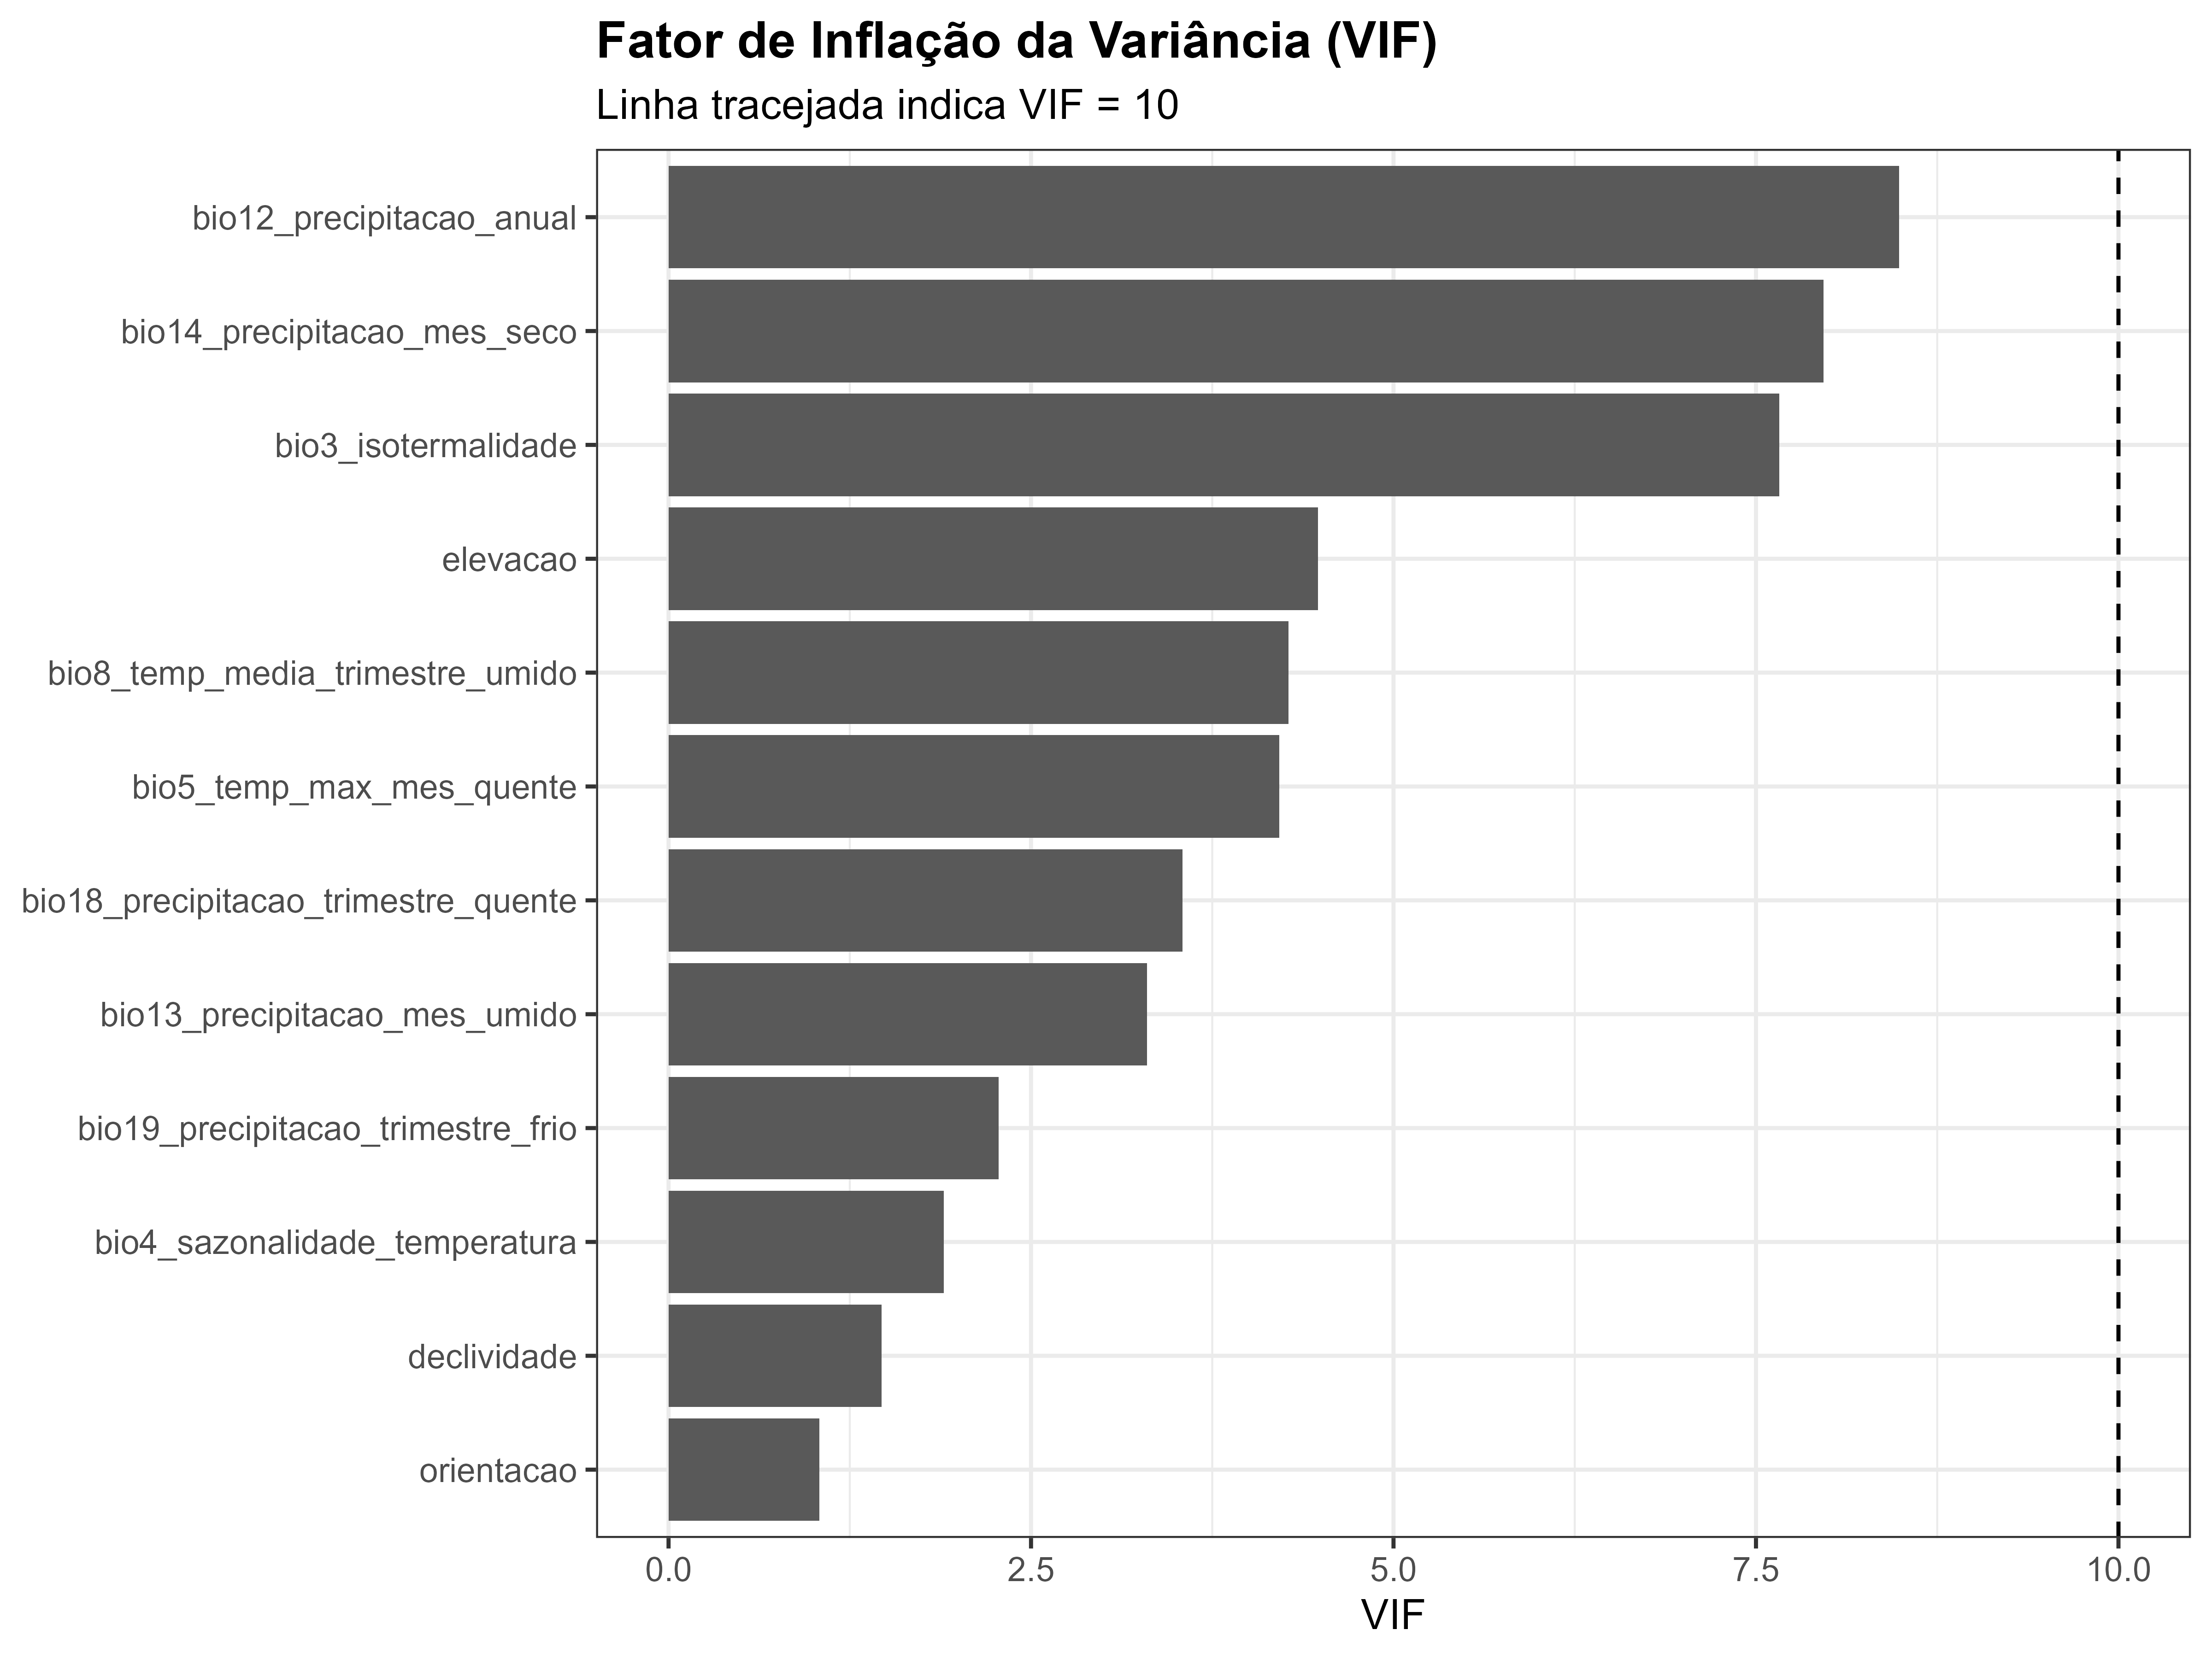
\includegraphics[width=0.92\textwidth]{figuras/unidade04/unidade04_vif_variaveis.png}
	\caption{Avaliação da multicolinearidade por meio do Variance Inflation Factor para as variáveis ambientais candidatas à modelagem de \textit{Dinizia excelsa}. Valores elevados indicam maior redundância em relação ao conjunto de preditores.}
	\label{fig:unidade04_vif_variaveis}
\end{figure}

As variáveis removidas foram aquelas que apresentaram redundância estatística elevada e menor contribuição interpretativa em relação às demais. Esse ponto é essencial: a remoção não significa que a variável seja ecologicamente irrelevante, mas que sua informação estava fortemente representada por outros preditores mantidos no conjunto final. Em SDM, essa distinção evita interpretações equivocadas, pois uma variável removida por multicolinearidade pode representar um processo importante, mas redundante dentro daquele conjunto ambiental específico.

\subsection{Análise de Componentes Principais}

A PCA foi utilizada como ferramenta complementar para compreender a estrutura multivariada do espaço ambiental. Diferentemente da matriz de correlação e do VIF, a PCA não foi usada diretamente como critério automático de seleção, mas como diagnóstico da organização dos gradientes ambientais. Ela permite visualizar quais variáveis contribuem para os principais eixos de variação e como os preditores se agrupam no espaço ambiental \parencite{dormann2013collinearity,franklin2010mapping}.

\begin{figure}[H]
	\centering
	\includegraphics[width=0.92\textwidth]{figuras/unidade04/unidade04_pca_variaveis.png}
	\caption{Análise de Componentes Principais das variáveis ambientais avaliadas para \textit{Dinizia excelsa}. A PCA auxilia na interpretação da estrutura multivariada do ambiente e na identificação de grupos de variáveis associadas aos principais gradientes ambientais.}
	\label{fig:unidade04_pca_variaveis}
\end{figure}

A interpretação da PCA ajuda a compreender se as variáveis finais representam dimensões ambientais complementares ou se permanecem concentradas em um único gradiente dominante. Para \textit{Dinizia excelsa}, o objetivo foi manter variáveis capazes de representar diferentes aspectos do espaço ambiental amazônico, evitando um conjunto dominado apenas por temperatura ou precipitação. Essa decisão aumenta a plausibilidade ecológica do modelo e favorece interpretações mais robustas nas unidades seguintes.

\subsection{Variáveis ambientais selecionadas}

A Tabela~\ref{tab:variaveis_selecionadas_final} apresenta o conjunto final de variáveis ambientais selecionadas para a modelagem de \textit{Dinizia excelsa}. O resultado final manteve nove variáveis, escolhidas por combinarem baixa redundância relativa, relevância ecológica e interpretabilidade. Esse conjunto será utilizado nas próximas unidades para geração de background, pseudo-ausências, calibração dos modelos e comparação entre algoritmos.

\begin{table}[H]
	\centering
	\caption{Variáveis ambientais selecionadas para a modelagem de \textit{Dinizia excelsa} após avaliação de correlação, VIF e interpretação ecológica. Esta tabela deve ser preenchida automaticamente a partir do arquivo \texttt{variaveis\_selecionadas\_final.csv}.}
	\label{tab:variaveis_selecionadas_final}
	\small
	\begin{tabular}{p{3.2cm}p{4.2cm}p{5.8cm}p{3.0cm}}
		\toprule
		\textbf{Variável} & \textbf{Tipo de gradiente} & \textbf{Interpretação ecológica} & \textbf{Decisão} \\
		\midrule
		\texttt{variavel\_01} & Climático/topográfico/edáfico & Descrição ecológica da variável selecionada & Mantida \\
		\texttt{variavel\_02} & Climático/topográfico/edáfico & Descrição ecológica da variável selecionada & Mantida \\
		\texttt{variavel\_03} & Climático/topográfico/edáfico & Descrição ecológica da variável selecionada & Mantida \\
		\texttt{variavel\_04} & Climático/topográfico/edáfico & Descrição ecológica da variável selecionada & Mantida \\
		\texttt{variavel\_05} & Climático/topográfico/edáfico & Descrição ecológica da variável selecionada & Mantida \\
		\texttt{variavel\_06} & Climático/topográfico/edáfico & Descrição ecológica da variável selecionada & Mantida \\
		\texttt{variavel\_07} & Climático/topográfico/edáfico & Descrição ecológica da variável selecionada & Mantida \\
		\texttt{variavel\_08} & Climático/topográfico/edáfico & Descrição ecológica da variável selecionada & Mantida \\
		\texttt{variavel\_09} & Climático/topográfico/edáfico & Descrição ecológica da variável selecionada & Mantida \\
		\bottomrule
	\end{tabular}
\end{table}

As nove variáveis finais foram mantidas porque, em conjunto, representam um espaço ambiental mais equilibrado e ecologicamente realista. Elas reduzem a duplicação de informação, preservam gradientes ambientais relevantes e permitem que os algoritmos posteriores sejam calibrados com menor risco de instabilidade. Essa decisão é particularmente importante para GLM e GAM, nos quais a interpretação dos coeficientes e curvas de resposta depende fortemente da estrutura dos preditores. Também é relevante para Random Forest, BRT e Maxent, pois variáveis redundantes podem afetar a importância relativa e a interpretação das respostas ambientais \parencite{elith2008working,dormann2013collinearity}.

Portanto, a seleção final não deve ser entendida como uma escolha meramente estatística, mas como uma síntese entre teoria ecológica, diagnóstico multivariado e objetivo de modelagem. Para \textit{Dinizia excelsa}, esse conjunto de nove variáveis servirá como base ambiental comum para as próximas etapas do livro, permitindo comparar algoritmos sob o mesmo espaço preditivo e avaliar como diferentes métodos traduzem os gradientes ambientais em mapas de adequabilidade.

\begin{caixaaplicacao}{Por que manter nove variáveis?}
	As nove variáveis finais foram mantidas porque representam um compromisso entre parcimônia e abrangência ecológica. Um número menor poderia simplificar excessivamente o nicho ambiental da espécie; um número maior poderia aumentar redundância e sobreajuste. O conjunto final busca representar os principais gradientes ambientais relevantes para \textit{Dinizia excelsa} sem duplicar informação de forma desnecessária.
\end{caixaaplicacao}

\section{Fluxograma de Seleção de Variáveis}

A seleção de variáveis ambientais pode ser compreendida como um fluxo de decisões sucessivas. Primeiro, parte-se de um conjunto amplo de variáveis candidatas. Em seguida, avaliam-se correlações entre pares de variáveis. Depois, aplica-se o VIF para identificar redundância multivariada. Na etapa seguinte, os resultados estatísticos são confrontados com o conhecimento ecológico da espécie. Por fim, define-se o conjunto final de variáveis a ser utilizado nos modelos.

\begin{figure}[H]
	\centering
	\includegraphics[width=0.92\textwidth]{figuras/unidade04/unidade04_fluxograma_vif.png}
	\caption{Fluxograma metodológico para seleção de variáveis ambientais em SDM. O processo combina diagnóstico estatístico e avaliação ecológica para obter um conjunto final de variáveis parcimonioso, interpretável e biologicamente plausível.}
	\label{fig:unidade04_fluxograma_vif}
\end{figure}

O fluxo apresentado na Figura~\ref{fig:unidade04_fluxograma_vif} resume a lógica adotada nesta unidade: Variáveis Brutas $\rightarrow$ Correlação $\rightarrow$ VIF $\rightarrow$ Avaliação Ecológica $\rightarrow$ Variáveis Finais. Essa sequência evita dois extremos metodológicos. O primeiro é incluir todas as variáveis disponíveis, prática que aumenta redundância e sobreajuste. O segundo é remover variáveis automaticamente sem considerar sua importância ecológica. A estratégia recomendada é equilibrar estatística e ecologia.

\section{Boas Práticas na Seleção de Variáveis}

A seleção de variáveis ambientais deve ser documentada de forma transparente. O leitor, o revisor ou outro pesquisador precisa compreender por que determinadas variáveis foram mantidas e por que outras foram removidas. Essa transparência aumenta a reprodutibilidade do estudo e fortalece a interpretação ecológica dos resultados. Em SDM, a qualidade metodológica não depende apenas do algoritmo utilizado, mas da coerência de todas as decisões tomadas antes da calibração do modelo \parencite{guisan2017habitat,zurell2020standard}.

\begin{table}[H]
	\centering
	\caption{Boas práticas para seleção de variáveis ambientais em Modelagem de Distribuição de Espécies.}
	\label{tab:boas_praticas_variaveis}
	\small
	\begin{tabular}{p{4.0cm}p{5.2cm}p{6.0cm}}
		\toprule
		\textbf{Situação} & \textbf{Problema} & \textbf{Recomendação} \\
		\midrule
		Uso de todas as variáveis disponíveis & Aumenta redundância, multicolinearidade e risco de sobreajuste & Realizar triagem por correlação, VIF e relevância ecológica \\
		Variáveis altamente correlacionadas & Dificultam interpretação e podem duplicar informação ambiental & Manter a variável com maior significado ecológico e melhor qualidade espacial \\
		Seleção puramente automática & Pode remover variáveis biologicamente importantes & Combinar diagnóstico estatístico com conhecimento ecológico da espécie \\
		Uso exclusivo de variáveis climáticas & Pode simplificar excessivamente o nicho de espécies vegetais & Avaliar inclusão de relevo, solos e outros preditores ecologicamente plausíveis \\
		Muitas variáveis derivadas da mesma base & Pode representar repetidamente o mesmo gradiente ambiental & Selecionar variáveis que representem dimensões ambientais distintas \\
		Variáveis difíceis de interpretar & Reduzem clareza ecológica e dificultam comunicação dos resultados & Priorizar variáveis com significado biológico claro \\
		Projeções futuras com variáveis instáveis & Reduzem transferibilidade e aumentam incerteza & Usar variáveis disponíveis e comparáveis nos cenários atuais e futuros \\
		Ausência de justificativa para variáveis mantidas & Compromete transparência e reprodutibilidade & Registrar critérios de seleção e decisões metodológicas \\
		Dependência excessiva de métricas de desempenho & Pode favorecer modelos estatisticamente bons, mas ecologicamente frágeis & Avaliar desempenho junto com plausibilidade ecológica e robustez \\
		Modelos comparativos com conjuntos diferentes de variáveis & Dificulta comparação entre algoritmos & Utilizar o mesmo conjunto ambiental final para todos os algoritmos principais \\
		\bottomrule
	\end{tabular}
\end{table}

Em síntese, boas práticas na seleção de variáveis envolvem parcimônia, coerência ecológica, controle de redundância, documentação transparente e compatibilidade com os objetivos do estudo. Para \textit{Dinizia excelsa}, essas boas práticas permitem construir um espaço ambiental sólido, que servirá como base para a geração de background e pseudo-ausências na próxima unidade e para a calibração dos modelos nas unidades seguintes.

\begin{caixaatencao}{Decisão metodológica consolidada}
	Neste livro, o conjunto final de nove variáveis ambientais selecionadas na Unidade 04 será utilizado como base comum para os modelos GLM, GAM, Random Forest, BRT, Maxent e Ensemble. Essa decisão garante comparabilidade entre algoritmos, reduz redundância e fortalece a interpretação ecológica dos resultados.
\end{caixaatencao}
